\documentclass[12pt]{article}

\usepackage[a4paper]{geometry}
\usepackage[utf8]{inputenc}
\usepackage[english]{babel}
\usepackage[automark]{scrpage2}
\usepackage{listings}
\usepackage{hyperref}
\usepackage{xcolor}
\usepackage{caption}
\usepackage{graphicx}

\pagestyle{scrheadings}
\clearscrheadfoot
\ihead[]{RoboSoccer Laboratory}
\ohead[]{Team C}
\cfoot[]{\pagemark}


\begin{document}

\section{Project plan}
\subsection{Definition of the project objectives}
The main project objective is winning the "RoboSoccer Championship" at the end of this course. 
This requires the implementation of low- and mid-level robot controls and an artificial intelligence with good tactics.

In addition the programm has to obey the RoboSoccer rules during the match and has to have a penalty-shoot-out mode.

\subsection{Framework and Procedure}
\subsubsection*{Hardware}
One team controlls three modded Pololu 3pi robots to shoot a golfball into the goal of the enemy.
They are connected to a server via bluetooth and located using a firewire camera above of the playground.

\subsubsection*{Team Members}
\begin{itemize}
	\item Markus Hofbauer
	\item He Jiang
	\item Kevin Meyer
	\item Benedikt Schmidt
	\item Florian Wirnshofer
\end{itemize}

\subsubsection*{Team Organisation}
\begin{itemize}
	\item \textbf{Internal Communication}
	\begin{itemize}
		\item Team Discussion Board \\\mbox{(phpBB: \textit{https://forum.kevin-meyer.de})}
		\item Email
	\end{itemize}
	\item \textbf{Weekly Jour Fixe} at Laboratory or Eikon
	\item Additional meetings on demand
\end{itemize}

\subsubsection*{Software}
\begin{itemize}
	\item \textbf{Target and Development-OS:} Linux
	\item \textbf{IDE:} Qt Creator
	\item \textbf{VCS:} Git (hosted on \textbf{bitbucket.org})
	\item \textbf{Build System:} CMake
\end{itemize}

\subsection{Tasks}
The project strategy is based on the spiral model with the following milestones:
\begin{itemize}
	\item \textbf{Deadline: \textcolor{red}{07.05.2014}}
	\begin{itemize}
		\item Kickoff Position
		\item Goalkeeper
		\item Penalty Shooting
	\end{itemize}
	
	\item \textbf{Deadline: \textcolor{red}{04.06.2014}}
	\begin{itemize}
		\item Collision Avoidance
		\item Ball Control
		\item Player Interaction
	\end{itemize}
	
	\item \textbf{Strategy and Tactics}\\
	\textbf{Deadline: \textcolor{red}{25.06.2014}}
	
	\item \textbf{RoboSoccer Championship}\\
	\textbf{Deadline: \textcolor{red}{02.07.2014}}
\end{itemize}

\subsection{Resource plan}
In addition to the standard responsibilities, every team member is responsible for special tasks:
\begin{itemize}
	\item \textbf{PM:} Benedikt Schmidt
	\begin{itemize}
		\item Communication with the contact person and the tutor of the course
		\item General team coordination
		\item Monitor realization of project plan
	\end{itemize}
	 
	\item \textbf{QM:} Florian Wirnshofer
	\begin{itemize}
		\item Ensure sufficient unit tests
		\item Continuous testing on hardware
		\item Balance quality aspiration and effort
	\end{itemize}
	
	\item \textbf{CM:} Kevin Meyer
	\begin{itemize}
		\item Ensure self-explaining and readable code style
		\item Supervise the documentation
		\item Maintain repository and discussion board
	\end{itemize}
	
	\item \textbf{SD:} Markus Hofbauer, He Jiang 
	\begin{itemize}
		\item Design and verify code structure
		\item Ensure building code
		\item Choose and connect external libraries
	\end{itemize}
	
\end{itemize}

\subsection{Time scedule}
% Split Gantt Chart into two pieces: 
% 21.04.14 - 25.05.14
% 26.05.14 - 29.06.14
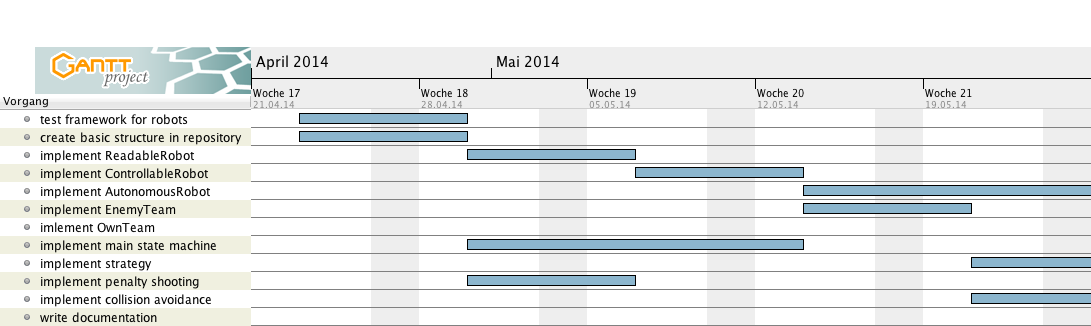
\includegraphics[width=\textwidth]{../ganttchart1.png}
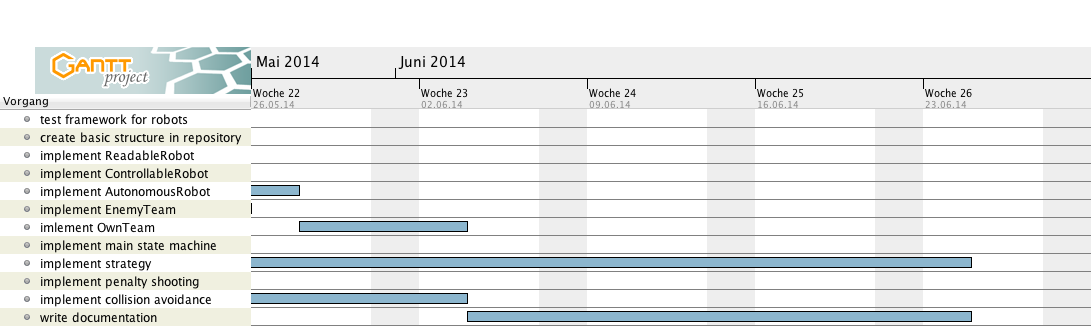
\includegraphics[width=\textwidth]{../ganttchart2.png}

\subsection{Cost plan}
In every Jour Fixe the team will discuss and create implementation issues, wich will be listed and managed inside bitbucket's issue tracker. 
Each team member will try to complete his assigned issues until the next jour fixe and report about it.

This will enable all team members a good knowlege of the current project status and a general insight about all project tasks. With this benefit it's easy to scale the effort needed for individual tasks, as they are hard to gauge at project start.

\subsection{Implementation}
Class diagramm: First draft\\
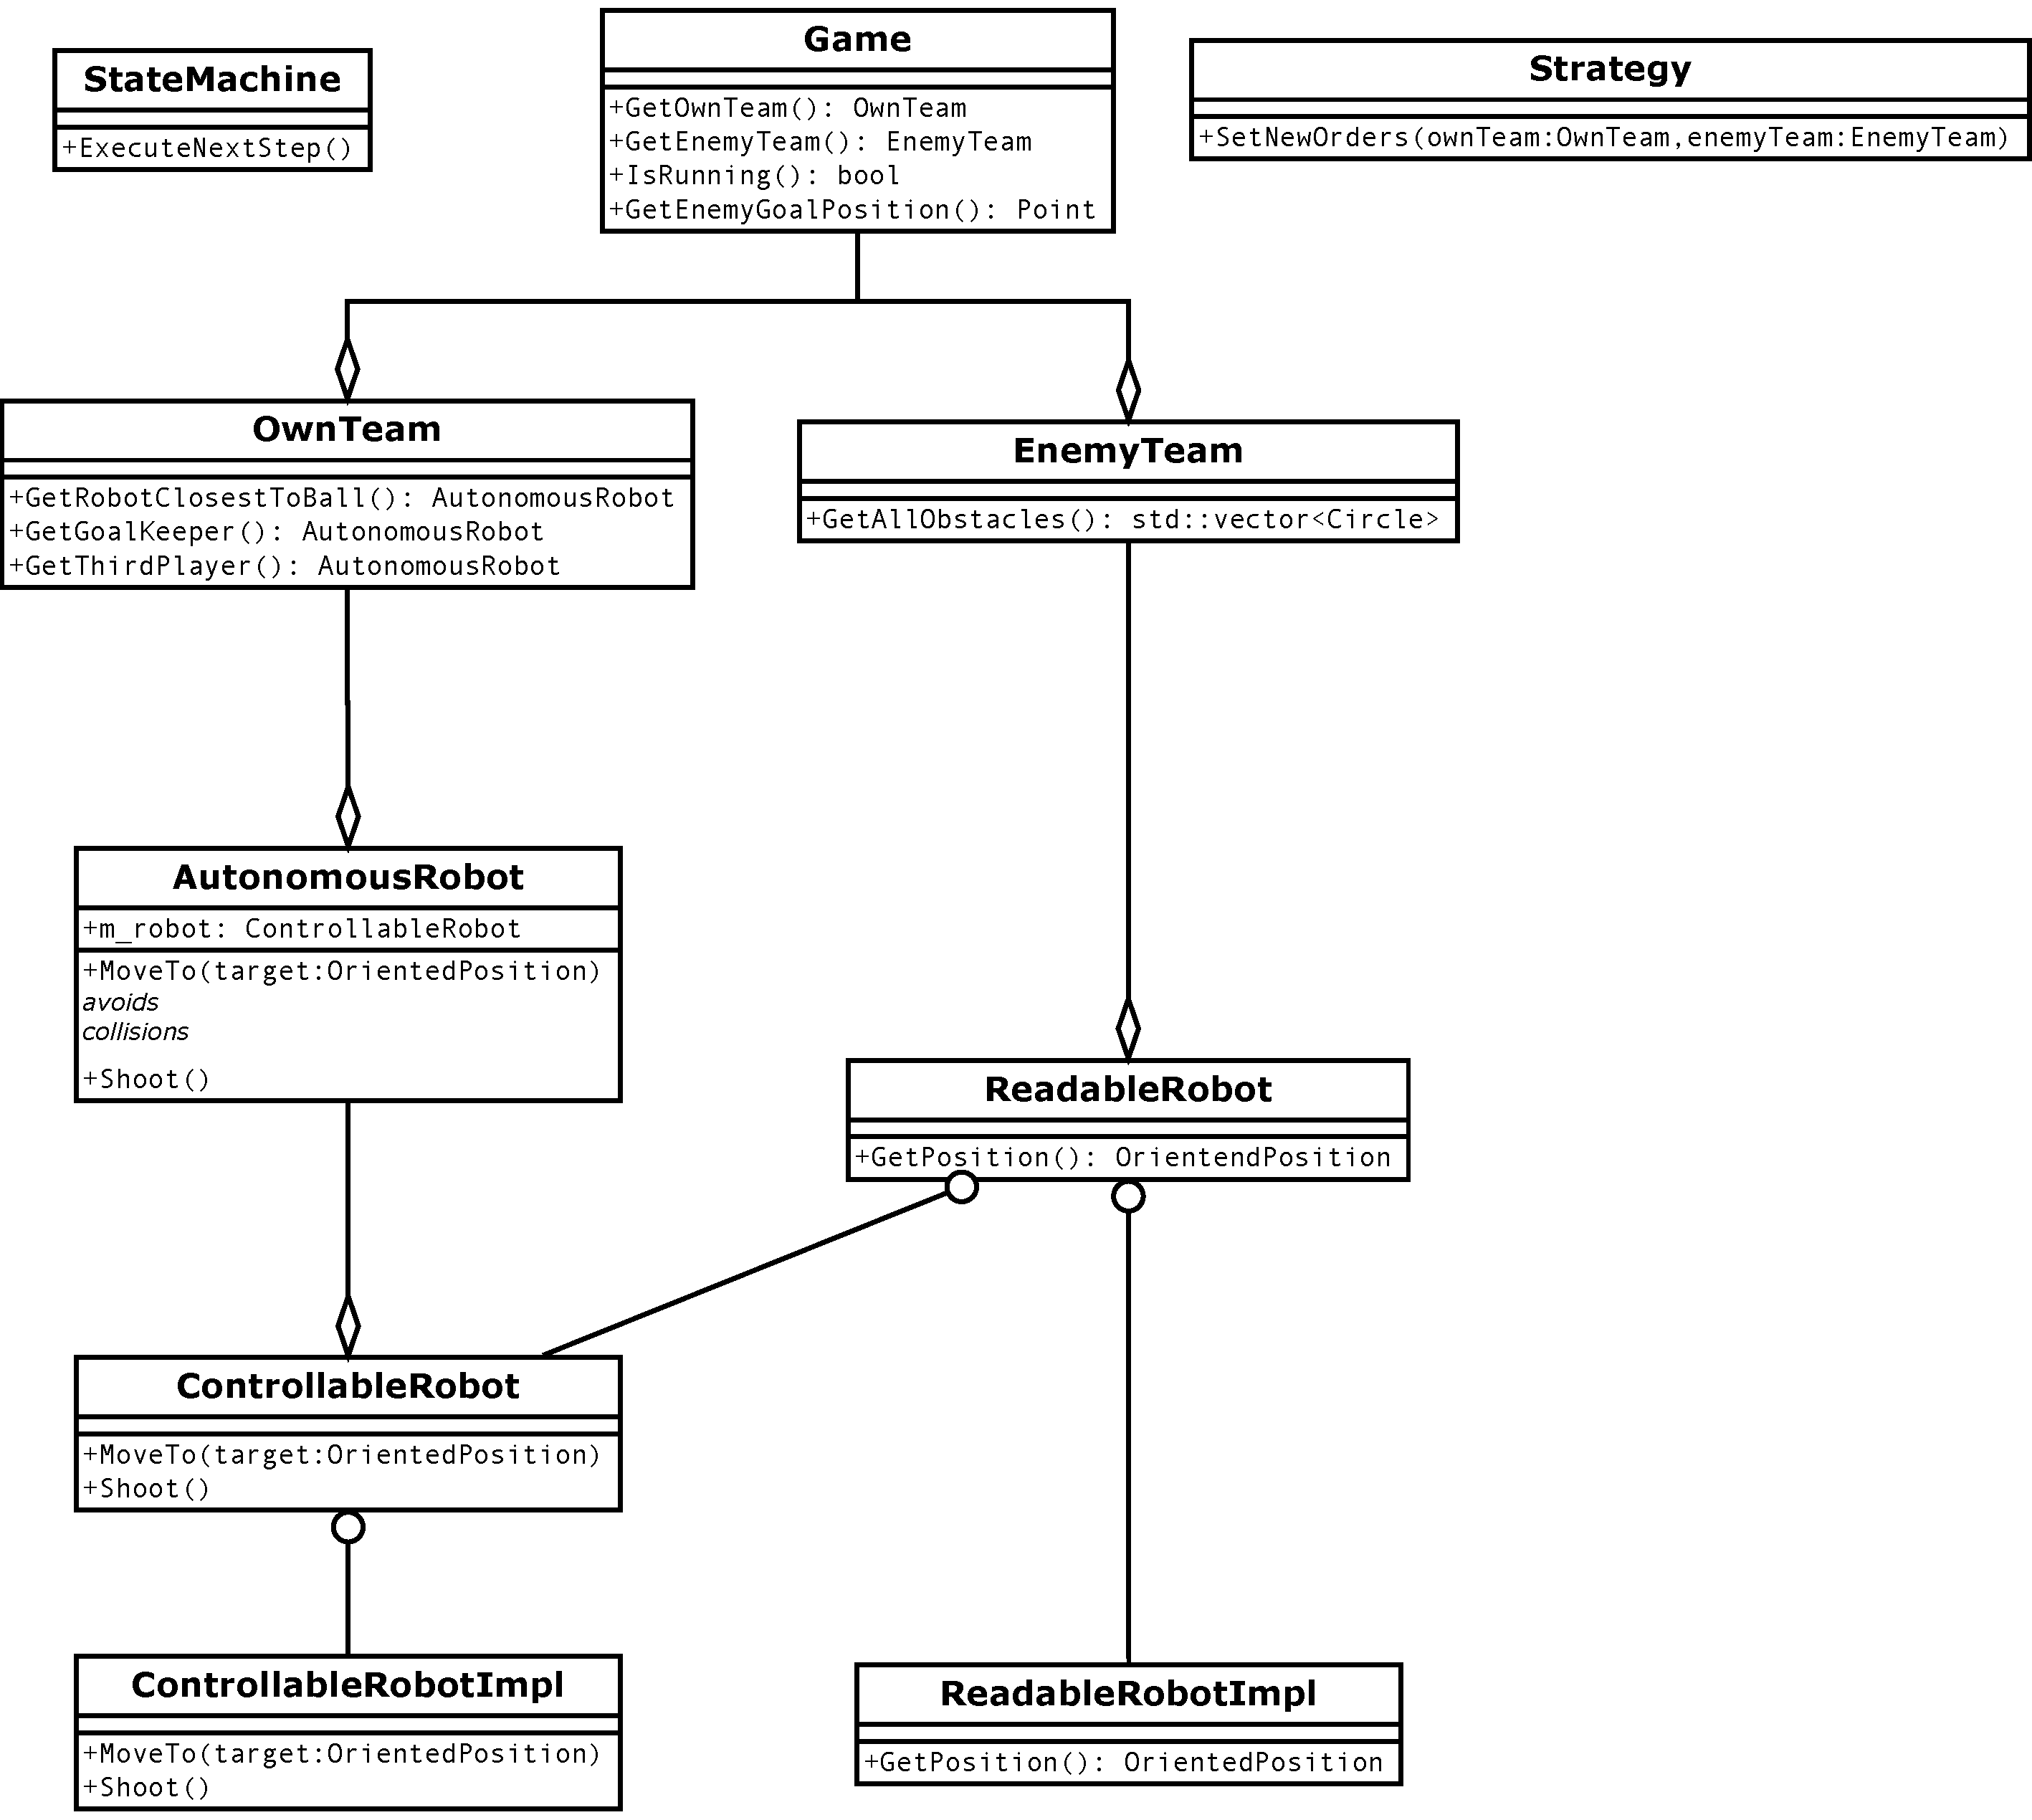
\includegraphics[width=\textwidth]{../architecture.pdf}

\end{document}
